\documentclass[a4paper,12pt]{article}

\usepackage[14pt]{extsizes}
\usepackage{cmap}					% поиск в PDF
\usepackage{mathtext} 				% русские буквы в формулах
\usepackage[T2A]{fontenc}			% кодировка
\usepackage[utf8]{inputenc}			% кодировка исходного текста
\usepackage[english,russian]{babel}	% локализация и переносы
\usepackage{graphicx}
\usepackage{geometry}
\usepackage{amsmath}
\usepackage[table]{xcolor}
\setlength\extrarowheight{2pt}


\geometry{verbose, a4paper, tmargin=2cm, bmargin=2cm, lmargin=3cm, rmargin=2cm}
\author{Vysotsky Maxim}
\title{Отчёт}
\date{2022}

\begin{document}
	\begin{titlepage}
		\begin{center}
			{Министерство науки и высшего образования Российской Федерации
				НАЦИОНАЛЬНЫЙ ИССЛЕДОВАТЕЛЬСКИЙ ТОМСКИЙ
				ГОСУДАРСТВЕННЫЙ УНИВЕРСИТЕТ (НИ ТГУ)}
		\end{center}
		\begin{center}
			{Физический факультет}
		\end{center}
		
		
		\vspace{8cm}
		{
			\begin{center}
				{\bf Лабораторная работа №2-3}\\
				Определение средней длины свободного пробега молекул газа
			\end{center}
		}
		\vspace{2cm}
		\begin{flushright}
			{Руководитель:\\ канд. физ.-мат. наук\\
				Конов И. А. \\
				Работу выполнили:\\
				Левин Н. Н. \\
				Высоцкий М. Ю.\\
				\vspace{0.2cm}
				гр. 052101}
		\end{flushright}
		\vspace{3cm}
		\begin{center}
			Томск, 2022
		\end{center}
	\end{titlepage}

\section{Теоретическое введение}
\textbf{Цель работы:} определение средней длины свободного пробега молекул газа.

\textbf{Длина свободного пробега молекулы } -- это среднее расстояние $\lambda$, которое пролетает частица за время между двумя последовательными столкновениями. Так как каждая молекула имеет собственное расстояние (т.е. для всех молекул оно различно), под длиной свободного пробега подразумевается именно среднее число $<\lambda>$.

Взаимодействие молекул в газе, молекулы которого находятся на относительно большом расстоянии друг от друга, носит характер столкновений. От частоты столкновений зависит время протекания процессов, ведущих к установлению состояния термодинамического равновесия: \textit{диффузии, теплопроводности, электропроводности}. Кроме того, от частоты соударений зависит протекание фазовых переходов в таких системах.

Чтобы определить частоту столкновений и длину свободного пробега допустим, что все молекулы \textit{покоятся}, а одна из них движется со скоростью $v$. Также примем диаметры всех молекул равными $d$, а концентрацию за $n$ (и так как виртуальная установка представляет собой двумерное пространство, концентрация будет относиться к единице площади, а не объема).

Частицы движутся, причем после каждого столкновения они меняют направление. Потому траектория, допусти, за 1 секунду, будет представлять собой ломаную линию. На Рис.1 изображена примерная траектория. Возле каждого излома линий будет стоять частица. Причем для того, чтобы летящая частица могла испытать с ней соударение, нужно чтобы центр неподвижной частицы попал между параллельными линиями.

\begin{figure}[h!]
	\begin{center}
		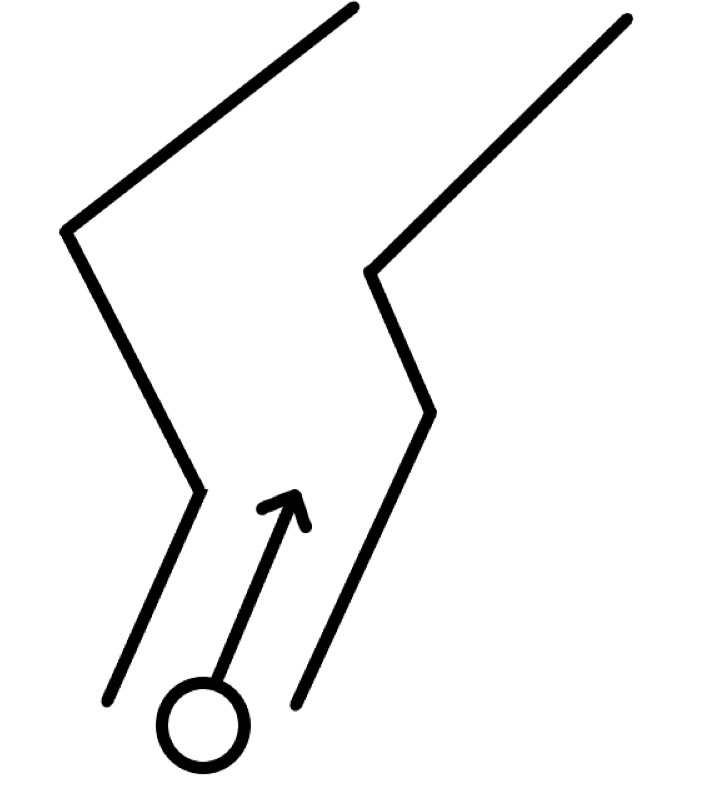
\includegraphics[scale=0.2]{1}
	\end{center}
	\caption{Примерная траектория полёта}
\end{figure}

\newpage

Вычислим число ударов, которые испытывает летящая частица за 1 секунду. За это время она проходит путь, равный скорости. Площадь, заключенная между параллельными линиями, приближенно равна произведению двойного диаметра на длину линии: $S = 2dv$. Число частиц $n$, находящихся на этой площади будет равно: $N = n2dv$. Эта величина равна числу столкновений выбранной молекулы с другими частицами за 1 секунду. Разделив её на путь $v$, получим выражение для средней длины свободного пробега:
\begin{equation}\label{rab_form}
\lambda = \frac{v}{N} = \frac{1}{2dn}
\end{equation}

Выражение \eqref{rab_form} получена в модели, в которой движется только сталкивающаяся молекула. Для реального движения других молекул вводится коэффициент $\sqrt2$ в знаменателе.

\newpage

\section{Ход эксперимента}
\hspace{\parindent}Для определения длины свободного пробега частицы была использована виртуальная установка. В ней нам предоставляется возможность выставлять необходимые значения количества частиц, а также их диаметра. 

Для начала мы определились с необходимым количеством соударений, а также начальными параметрами системы: количество соударений -- 50, $N$ = 20, $d$ = 15. 

После этого, посредством нажатия кнопки <<Пуск>>, мы стали дожидаться момента, когда количество соударений станет равным 50. Соответствующее значение, а также среднюю длину свободного пробега, экспериментальная установка выводит на экран. 

Далее, соответствующий опыт был проведен для других значений $N$. Результаты измерений представлены в таблице ниже:
\begin{center}
	\begin{tabular}{|c|c|c|}
		\hline
		$Соудар$&		$N$&		$ср$\\
		\hline
		50&		5&		1098\\
		\hline
		50&		10&		376\\
		\hline
		50&		15&		288\\
		\hline
		50&		20&		255\\
		\hline
		50&		25&		187\\
		\hline
		
	\end{tabular}
\end{center}

Используя полученные данные, мы построили график зависимости средней длины свободного пробега от количества частиц.

\begin{figure}[h!]
	\begin{center}
		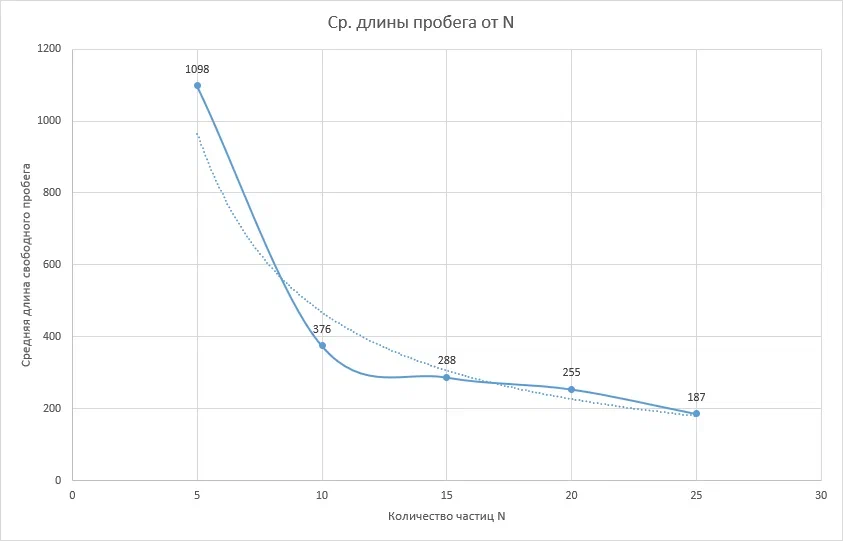
\includegraphics[scale=0.4]{2}
	\end{center}
	\caption{График зависимости средней длины свободного пробега от количества частиц}
\end{figure}

\newpage
Проанализировав данный график, мы можем сказать, что он отдалённо напоминает гиперболу в первой четверти координатной плоскости, о чём также свидетельствует вид формулы \eqref{rab_form}.

Мы посмотрели на поведение системы при фиксации параметра $d$, что и позволило нам отследить зависимость представленную выше. Далее, в ходе эксперимента, мы произвели те же действия, но при фиксированном параметре $N$, что позволило определить зависимость средней длины свободного пробега от диаметра частиц. Полученные результаты и соответствующий график представлены ниже:
\begin{center}
	\begin{tabular}{|c|c|c|}
		\hline
		Соудар&		d&		ср\\
		\hline
		50&		5&		2350\\
		50&		10&		546\\
		50&		15&		315\\
		50&		20&		148\\
		\hline
	\end{tabular}
\end{center}

\begin{figure}[h!]
	\begin{center}
		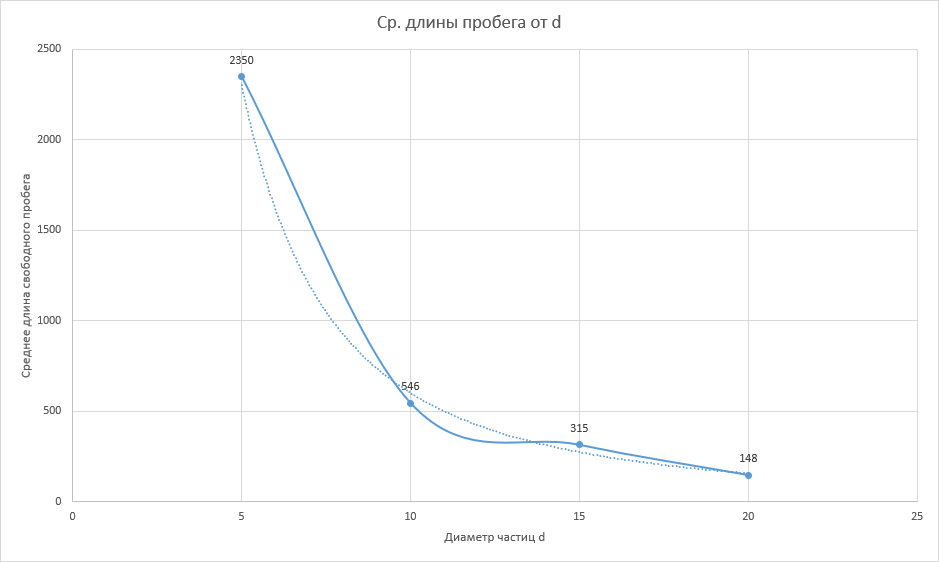
\includegraphics[scale=0.4]{3}
	\end{center}
	\caption{График зависимости средней длины свободного пробега от диаметра частиц}
\end{figure}

Данный график, так же как и предыдущий, отдалённо напоминает гиперболу в первой четверти координатной плоскости.

\newpage
\section{Вывод}
\hspace{\parindent}В первую очередь, необходимо сделать уточнение, что данная работа опирается на предположение, что рассматриваемый газ является идеальным. Следовательно, справедливы утверждения, что между молекулами отсутствуют силы взаимодействия; молекулы принимаются за материальные точки; соударения молекул подчиняются закону упругих соударений.

В данной работе средняя длина свободного пробега молекулы определялась автоматически - виртуальной установкой. Вследствие чего определение прямых и косвенных погрешностей не представляется возможным.

При анализе первого и второго графиков, мы подобрали наиболее подходящую под данный тип зависимости линию тренда - степенная функция. Вследствие чего мы можем сказать, что средняя длина свободного пробега частицы, что в первом, что во втором случаях, представляет собой степенную зависимость - это наблюдается как алгебраически в рабочей формуле \eqref{rab_form}, так и графически.

Также следует заметить, что при зависимости средней длины свободного пробега частицы от диаметра молекул (второй график), первая величина убывает быстрее с ростом $d$, по сравнению с зависимостью от количества молекул.


\end{document}